\documentclass[11pt, a4paper]{article}
\pdfminorversion 5
\usepackage{varioref}
% fancyheadings: Fancy headers
\usepackage{fancyhdr}
% avantgar, chancery, charter, courier, helvetic, newcent, pandora,
% palatino, times, utopia, zapfchan: Fonte
% euler: Math font
\usepackage{palatino}
\usepackage{upgreek}
%\usepackage{newcent}
% listings: For listing code with syntax highlighting
\usepackage{listings}
% graphicx: Include graphic-files
\usepackage{graphicx}
\usepackage{subfigure}
%\usepackage{wrapfig}
% amsmath: more mathcommands
%\usepackage{amsmath}
%\usepackage{amssymb}
%\usepackage{amsthm}
% a4wide: for longer lines
%\usepackage{a4wide}
% Package for infix arithmetic notation
\usepackage{calc}
% Defines if/then/else macros for conditional text
\usepackage{ifthen}
% Place selected parts of a document in landscape
\usepackage{verbatim}

\usepackage{url}

\usepackage{todonotes}

\usepackage{listings}

\usepackage{amsmath}

\usepackage{clrscode}

\usepackage[standard,thmmarks]{ntheorem}


%------------------------------------------------------------
% Setting up the ntheorems
%------------------------------------------------------------
% Examples
\theoremstyle{plain}
\theorembodyfont{\upshape}
\theoremsymbol{\ensuremath{\ast}}
\theoremseparator{}
\renewtheorem{Example}{Example}

\theoremstyle{empty} 
\theorembodyfont{\upshape}
\theoremsymbol{\ensuremath{\ast}}
\theoremseparator{}
\newtheorem{contexampleinner}{} 

\newenvironment{contExample}[1]{% 
\begin{contexampleinner}[Example~\ref{#1} 
(Continued)]}{\end{contexampleinner}} 

% Definitions
\theoremstyle{plain}
\theoremsymbol{\ensuremath{\clubsuit}}
\theoremseparator{.}
\theoremprework{\bigskip\hrule}
\theorempostwork{\hrule\bigskip}
\renewtheorem{Definition}{Definition}


%------------------------------------------------------------
% Set up listings environment
%------------------------------------------------------------
%\lstloadlanguages{}
\makeatletter
\lstset{
  columns=fullflexible,
  basicstyle=\ttfamily\small,
  keywordstyle=\bfseries,
  commentstyle=\itshape,
  showstringspaces=f,
  keepspaces=true,
  numbers=left, 
  numberstyle=\tiny, 
  stepnumber=2, 
  numbersep=5pt, 
  language=C,
}
\makeatother

%------------------------------------------------------------
% Set up headers and footers
%------------------------------------------------------------
\pagestyle{fancy}
\fancyhead{}
% Put pagenumber centered on bottom of page
\lfoot{}
\cfoot{\thepage}
\rfoot{}
% Put section number and name on top left of page
\renewcommand{\sectionmark}[1]{\markboth{\thesection\ #1}{}}
\lhead{\fancyplain{}{\leftmark}}
% Make sure the rest is blank
\chead{}\rhead{}


%------------------------------------------------------------
% My own lists
%------------------------------------------------------------
\newlength{\Mylen}
\newcommand{\entrylabel}[1]{%
  \settowidth{\Mylen}{#1}%
  \ifthenelse{\lengthtest{\Mylen > \labelwidth}}%
  {\parbox[b]{\labelwidth}%
    {\makebox[0pt][l]{#1}\\}}%
  {#1}%
  \hfil\relax}
\newenvironment{entry}
{\begin{list}{}%
    {\renewcommand{\makelabel}{\entrylabel}%
      \setlength{\labelwidth}{35pt}%
      \setlength{\leftmargin}{\labelwidth+\labelsep}%
    }%
  }%
{\end{list}}

\title{Speciale}
\author{Line Bie Pedersen 300976}
\date{}

\begin{document}
\maketitle

\section*{Abstract}

\tableofcontents

\section*{List of Examples}

\theoremlisttype{all}
\listtheorems{Example}

\section{Introduction}
%\todo[inline]{jan: Before this section, you should have a separate, uncounted, page thanking those that have helped you.}
Regular expressions is an important tool for matching strings of
text. In many text editors and programming languages they provide a
concise and flexible way of searching and manipulating text. They find
their use in areas like data mining, spam detection, deep packet
inspection and in the analysis of protein sequences, see
\cite{pedersen2010}.

This masters thesis presents a design and an implementation of a
regular expression engine with focus on memory consumption. Also 
included is an evaluation of the work and a discussion about possible
future extensions.



\subsection{Motivation}

Regular expressions is a popular area in computer science and has seen
much research. They are used extensively both in academia and in
business. Many programming language offer regular expressions in some
form, either as an embedded feature or as a stand alone
library. There are many different flavors of regular expression and
implementations, each adapted to some purpose. 

\paragraph{Challenges and desired outcome}
Many of the existing solutions gives no guarantees on their memory
consumption. In this project we will focus on a streaming solution,
that is we will, where possible, use a constant amount of memory for a
fixed regular expression. We will build a general framework to this
purpose. In addition we wish to attempt to isolate the steps taken in
matching a regular expression with a string. We do this because we can
then plug in exactly the steps needed for a particular operation and
leave out the rest. Another reason for doing this is that, it is then
possible to isolate the trouble spots where optimization is most
needed. 


%In addition, we wish to attempt to isolate each regular expression step \todo{jan: finish with why}


%These improvements should be particular useful in situations where ...\todo{jan: write something about where ;)}

%% Regular expressions has seen much research. Det er brugt mange steder
%% i erhvervslivet. Mange programmeringssprog tilbyder regulære udtryk,
%% enten indbygget eller som et seperat bibliotek. DEr findes mange
%% forskellige modeller tilpasset diverse formål. 

%% I det her projekt vil vi forsøge at at løse problemet ved at bruge
%% konstant hukommelse(fraregnet pladsen til det regulære udtryk). Mange
%% af de prodrukter der eksisterer idag giver ingen garantier på
%% hukommelsesforbruget. Vi vil forsøge at stille et generelt framework
%% op som kan løse dette


\subsection{Definitions, conventions and notation}

The empty string is denoted as $\upvarepsilon$. $\Sigma$ is used to
denote the alphabet, or set of symbols, used to write a string or a
regular expression. 

Automatons are represented as graphs, where states are nodes and
transitions are edges. The start state has an arrow starting nowhere
pointing to it. The accepting state is marked with double
circles. Edges has an attached string, indicating on which input
symbol this particular transition is allowed.

Regular expressions will be written in sans serif font:
\textsf{a\textbar b} and strings will be written slanted: \textsl{The
  cake is a lie}.


\subsection{Objectives and limitations}

The objectives of this thesis is to extend existing theory and design,
implement and evaluate a prototype. We will be extending theory by
Dub\'{e} and Feeley \cite{Dube2000} and Henglein and Nielsen
\cite{Henglein2010}. The extended theory will be used in designing a
streaming regular expression engine. The design will be implemented in
a prototype and finally we will evaluate and compare with existing
solutions.

We aim to address these topics in this thesis:

\begin{itemize}
\item Extend existing theory by Dub\'{e} and Feeley \cite{Dube2000}
  and Henglein and Nielsen \cite{Henglein2010}.

\item Create a prototype implementation

\item Compare the prototype with existing solutions and evaluate our own results

\item Conclude, and propose extensions and improvements on the work
\end{itemize}

\subsubsection{Limitations}

The focus is on designing and implementing a streaming regular
expression engine. There are many general purpose features and
optimizations that can be considered necessary in a full-fledged
regular expression engine but that we only consider peripherally
here. In situations where we are faced with a choice, we have
generally favored simplicity and robustness.  In several cases, we
only theoretically discuss alternative solutions and do not provide a
prototype.%\todo{jan: Ok?}
%% Fokus på at bevise ideen ikke et stort featuresæt, den kan ikke serach
%% and replace

\subsubsection{Implementation Choices}
Some choices were made early in the planning phase. This includes the
choice of programming language. There are several good reasons for
choosing C: We have previous experience developing in this language,
it has a low memory and run time overhead and libraries are well
documented and tested. The obvious drawback of using C is, as always,
that it is a primitive language, making it a time consuming process
developing new programs compared to other more high level languages.

Similarly, we chose to develop the program on a Linux platform for two
reasons; first, it is a natively supported platform for many other regular
expression libraries, which makes comparisons simpler, and lastly for
practical purposes, it is a free and highly rich platform that the
authors were already familiar with.


%% Some choices were made quite early in the planning phase. This
%% includes choice of programming language, where C was chosen for two
%% main reasons: it provided a good baseline comparison against other
%% implementations (with a minimal library and memory overhead compared
%% to many other languages) and while it was not necessary to reuse
%% code\todo{jan: er det sandt?}, we already had good experiences using C
%% from earlier experiments with regular expressions. The obvious
%% drawback to C is that it is often more time consuming to develop
%% software due to the relative primitiveness of the language and
%% library.

Other choices that were made early was to build on the work of
Dub\'{e} and Feeley and Henglein and Nielsen, especially for the mixed
bit-values concept. This will be treated in more detail later.
%% =======
%% \todo[inline]{jan: Mest filler så dette her kapitel ikke var så kort, men du manglede det vist}
%% Some choices were made quite early in the planning phase. This includes choice of programming language, where C was chosen for two main reasons: it provided a good baseline comparison against other implementations (with a minimal library and memory overhead compared to many other languages) and while it was not necessary to reuse code\todo{jan: er det sandt?}, we already had good experiences using C from earlier experiments with regular expressions. The obvious drawback to C is that it is often more time consuming to develop software due to the relative primitiveness of the language and library.

%% Similarly, we chose to develop the program on a POSIX (specifically Linux) platform for two reasons; first, it is the primary platform for many other regular expression libraries, which makes comparisons simpler, and lastly for practical purposes, it is a free and highly rich platform that the authors were already familiar with.

%% Other choices that were made early was to build on the work of Henglein and Nielsen, especially for the mixed bit values concept. This will be treated in more detail later.
%% >>>>>>> 70e74b980e010e636dc9303698dd72c89196b3c3

\subsection{Summary of contributions}

The main contribution of this thesis work is a streaming regular
expression engine based on Dub\'{e} and Feeley \cite{Dube2000} and
Henglein and Nielsen \cite{Henglein2010}. We present, implement and
evaluate a working prototype that demonstrates that our solution is
both technically viable and in many cases preferable from a
resource-consumption standpoint compared to existing industry
solutions.

\subsection{Thesis overview}

Section \ref{sec:regular_finite} gives an introduction to regular
expressions and finite automatons. In section \ref{sec:design} we
describe the architecture of our implementation. Section
\ref{sec:implementation} has the implementation specific details. In
section \ref{sec:optimizations} we describe the behavior of the
implemented prototype, suggest some optimizations and describe how we
implemented some of them. In section \ref{sec:theoretical} we have the
complexity analysis. Section \ref{sec:evaluation} compares our
implementation to existing implementations. In section
\ref{sec:related} we have the related work. Section \ref{sec:future}
describes future work, improvements to the design and the
implementation of the prototype. Lastly we have the conclusion on our
theoretical and practical work in section \ref{sec:conclusion}.

%\cite{Cox2007}

\section{Regular expressions and finite automatons}
\label{sec:regular_finite}
%% \todo[inline]{MAn bruger dem til at beskrive tekststrenge med bestemte
%% mønstre, prøv at sætte noget lettere fordøjeligt ind før definitionerne}

A regular language is a possibly infinite set of finite sequences of
symbols from a finite alphabet. It is a formal language that must
fulfill a number of properties.

%\todo{wikipedia havde noget interessant at sige men vi kan ikke bare
%  kopiere det ind :(}

We provide this formal definition of regular languages:
\begin{definition}[Regular language]
  The regular language over the alphabet $\Sigma$ is defined
  recursively as:
  \begin{itemize}
  \item The empty language $\emptyset$.
  \item The empty string language $\{\upvarepsilon\}$.
  \item The singleton language $\{a\}$, for any symbol $a\in \Sigma$.
  \item If $L_r$ and $L_s$ are both regular languages then the union
    $L_r \cup L_s$ is also a regular language.
  \item If $L_r$ and $L_s$ are both regular languages then the
    concatenation $L_r \bullet L_s$ is also a regular language.
  \item if $L$ is a regular language then the Kleene star\footnote{We use the conventional definition of the Kleene star; a unary operator meaning ``zero or more'' } $L*$ is also
    a regular language.
  \end{itemize}
\end{definition}



\subsection{Regular expressions}

Regular expressions are used to denote regular languages. They are
written in a formal language consisting of two types of characters:
meta, and literal characters. The meta characters have
special meaning and are interpreted by a regular expression
engine. Some of the basic meta characters include parenthesis, the alternation
operator and the Kleene star. Parenthesis provides grouping,
alternation allows the choice between different text strings and the
Kleene star repeats. 

The literal characters have no special meaning; they simply match literally.

%% \begin{definition}[Regular language]
%% A regular language over the alphabet $\Sigma$ can be defined
%% recursively as follows:
%% \begin{description}
%% \item[Basis clauses] 
%%   \begin{itemize}
%%   \item The empty language $\emptyset$
%%   \item The empty string language $\{\upvarepsilon\}$
%%   \item The singleton language $\{a\}$, for any symbol $a\in \Sigma$
%%   \end{itemize}
%%   are all regular languages
%% \item[Inductive clauses]
%%   If $L_r$ and $L_s$ are both regular languages then
%%   \begin{itemize}
%%   \item The union $L_r \cup L_s$
%%   \item The concatenation $L_r \bullet L_s$
%%   \item The kleene star $L_r*$ 
%%   \end{itemize}
%%   are all regular languages
%% \item[Extremal clause] No other languages over $\Sigma$ are regular
%% \end{description}
%% \end{definition}

%% Regular expressions are used to regular languages:

A formal definition of regular expressions:
\begin{definition}[Regular expression]
  \label{def:regexp}
  A regular expression over an alphabet $\Sigma$ can be defined as follows:
\begin{itemize}
\item An empty string, $\upvarepsilon$, and any character from the
  alphabet $\Sigma$
\item If $r_1$ and $r_2$ are regular expressions, then the
  concatenation $r_1r_2$ are also a regular expression
\item If $r_1$ and $r_2$ are regular expressions, then the alternation
  $r_1|r_2$ is also a regular expression
\item If $r$ is a regular expression, then so is the repetition $r*$
\end{itemize}

Any expression is a regular expression if it follows from a finite
number of applications of the above rules.
\end{definition}

The precedence of the operators are: repetition, concatenation and
alternation, from highest to lowest. Concatenation and alternation are
both left-associative. 

\begin{example}[Regular expression]
  Here we have a somewhat complicated example of a regular expression
  that demonstrates the basic operators.
\label{ex:regular1}
Consider the sentence:
\begin{quote}
\textsl{This book was written using 100\% recycled
  words.}\footnote{Terry Pratchett, Wyrd Sisters}
\end{quote}

Other writings such as papers and novels also use words. If we
want to catch sentences referring to these writings as well, we can
use the regular expression: \texttt{(book|paper|novel)}. 

To match the number 100 in the sentence, we could use the regular
expression \texttt{100}. In most cases however we will not know
beforehand how many words are recycled, so we may want to use the
regular expression \texttt{(0|1|2|3|4|5|6|7|8|9)*}, which will match
any natural number.

With this in mind we can write a regular expression to match our
sentence:
\begin{quote}
  \texttt{This (book|paper|novel) was written using \\
    (0|1|2|3|4|5|6|7|8|9)*\% recycled words.}
\end{quote}

\end{example}

\subsection{Extensions to the regular expressions}

Many tools extend the regular expressions presented in the previous
section. A typical extensions is new notation to make it easier to specify
patterns. In this section we present the extensions to definition
\vref{def:regexp} we have made: Additional quantifiers, character classes,
a quoting symbol, a wild card and non-capturing parenthesis.

\begin{itemize}
\item The quantifier $+$ causes the regular expression $r$ to be
  matched one or more times. This can also be written as $rr*$
\item The quantifier $?$ causes the regular expression $r$ to be
  matched zero or one times. This can also be written as
  $\upvarepsilon|r$
\item A character class is delimited by $[]$ and matches exactly one
  character in the input string. Special characters loose their
  meaning inside a character class; $*$, $+$, $?$, $($, $)$ and so on
  are treated as literals.

  Characters can be listed individually, e.g. \texttt{[abc]}, or they
  can be listed as ranges with the range operator: $-$,
  e.g. \texttt{[a-z]}. These can be rewritten in terms of our original
  regular expression: \texttt{a|b|c} and \texttt{a|b|c...x|y|z}
  respectively.

  To match characters not within the range, the complement operator is
  used. \texttt{\^{}} used as the first character in a character
  class, elsewhere it will simply match literally, indicates that only
  characters not listed in the character class should
  match. E.g. \texttt{[\^{}\^{}]} will match anything but a
  \texttt{\^{}}
\item The quoting character \textsf{\textbackslash} will allow the
  operators to match literally. We use \textsf{\textbackslash *} to
  match a \textsl{*}.
\item The wild card \texttt{.} will match any character, including a
  newline.
\item For the non-capturing parenthesis we have the choice of
  notation. Here we will list some of the options, where $r$ is some
  regular expression:
  \begin{itemize}
  \item The industry standard, to which Perl, Python, RE2 and most
    others adhere is: $(?:r)$.
  \item Perl 6 \cite{Wall2002} suggests use of square parenthesis instead:
    $[r]$. These are however already in use by the character classes.
  \item A more intuitive notation could be using single parenthesis
    for non-capturing, $(r)$, and double parenthesis for capturing,
    $((r))$.
  \item A currently unused option is $\{r\}$ as special notation,
    which would be simple to implement. This is however the industry
    standard for repetition notation.
  \end{itemize}
  
  Since there is a standard, we will adhere to it, and use $(?:r)$ for
  non-capturing parenthesis.
\end{itemize}
\begin{example}

As we saw in example \ref{ex:regular1}, we can match a natural number
with the regular expression \texttt{(0|1|2|3|4|5|6|7|8|9)*}. Using the
expansions to regular expressions above, we can rewrite this as:
\begin{description}
\item[\texttt{[0-9]*}] This literally means the same thing.
\item[\texttt{[0-9]+}] We can use a different repetition operator and
  require there be at least one digit.
\item[\texttt{[1-9][0-9]*}] This matches any natural number as
  well, but it will not match any preceding zeros. This is a
  refinement, in that it will match fewer text strings than the first
  expression. It is up to the expression writer to decide what the desired outcome is.
\end{description}
\end{example}


\subsection{Finite automatons}

Finite automatons are used to solve a wide array of problems. In this
thesis we will focus on finite automatons as they are used with
regular expressions. 
A finite state machine consists of a number of
states and transitions between states. It is constructed as follows:
\begin{itemize}
    \item One state is marked as the
    initial state
    \item a set of states, one or more, is marked as final
    \item A condition is attached to each transition between states
    \item Input is consumed in sequence and for each symbol transitions are taken when their attached condition are met
    \item If the simulation ends in a final state, the finite automaton is said to accept the input
\end{itemize}

Finite automatons can be divided in two main categories: The
deterministic (DFA) and the non-deterministic (NFA) finite
automaton. This distinction is mostly relevant in practice, as they
are equivalent in terms of computing power. NFAs and DFAs recognize
exactly the regular languages.

%% \todo[inline]{jan: What about "Nondeterministic finite automata with
%%   epsilon-transitions (FND-epsilon or epsilon-NFA)"}


\begin{description}
\item[NFA] For each pair of input symbol and state, there may be more
  next states. This means that there may be several paths through an
  NFA for a given input string.

  The $\upvarepsilon$-transitions are an extension of the NFA. These
  are special transitions that can be taken without consuming any
  input symbols. This also has mainly practical implications, NFAs
  with and without $\upvarepsilon$-transitions are equivalent.

\item[DFA] For each pair of input symbol and state, there may be only
  one next state. This means there is only one path through the DFA
  for a given input string.
\end{description}

The advantage of a NFA is the size, the number of states and
transitions in a NFA is linear in the size of the regular expression,
whereas a DFA will in the worst case have a number of states
exponential in the size of the regular expression. The advantage of a
DFA is the effort required to simulate it. It only requires time
linear in the size of the input string and constant space (not
counting the space for the DFA), whereas the NFA requires time linear
in the product of the size of the regular expression and input string
and space linear in the size of the regular expression.

%% \todo[inline]{jan: Aren't you forgetting the size growth of either?
%%   Also you're not talking about the properties of either, and their
%%   respective disadvantages}


\subsection{Regular expression to NFA}
\label{sec:from_regular_expression_to_nfa}
Every regular expressions can be converted to a NFA matching the same
language.  This section will describe an approach to doing so.

\subsubsection{Thompson}
\label{sec:re2nfa_thompson_theory}
The method described in this section first appeared in Ken Thompsons
article from 1968 \cite{Thompson1968}. The descriptions given in for
example \cite{HopcroftJohnE.AndMotwaniRajeevAndUllman2001},
\cite{Aho:1986:CPT:6448} and \cite{RussCox} are considered more
readable and we will be basing our description on these.

The NFA will be build in steps from smaller NFA fragments. A NFA
fragment has an initial state, but no accepting state, instead it has
one or more dangling edges leading nowhere (yet).


%% a method for converting a
%% regular expression to an automaton is described. The method works by
%% breaking the regular expression up into fragments; Each fragment also
%% being a regular expression in itself. Using this method yields an
%% automaton with the following characteristics:
%% \begin{itemize}
%% \item There is exactly one initial state
%% \item There are no edges into the initial state
%% \item There is exatly one accepting state
%% \item There are no edges out of the accepting state
%% \item There are at most two edges leaving a state
%% \end{itemize}

The base fragment corresponds to the regular expression consisting
only of a single character \textit{a}. The NFA fragment is shown in
figure \vref{fig:basecase1}. One state with a single edge, marked with
the character \textit{a} is added. The new state is the initial state
for this fragment and the edge is left dangling.

\begin{figure}
  \centering
  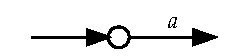
\includegraphics{parsing/basecase1}
  \caption{Fragment accepting a single character \textit{a}}
  \label{fig:basecase1}
\end{figure}

The second base fragment corresponds to the empty regular
expression. The NFA fragment is shown in figure
\vref{fig:basecase4}. One state with a single edge marked as a
$\upvarepsilon$-edge is added. The new state is the initial state for
this fragment and the edge is left dangling. This fragment is used for
the empty regular expression and for alternations with one or more
options left empty.

%% In Ken Thompson article from 1968 \cite{Thompson1968}, in
%% \cite{HopcroftJohnE.AndMotwaniRajeevAndUllman2001} and in
%% \cite{RussCox} a method for converting a regular expression to an
%% automaton is described.



%% The base case is the regular expression consisting of a single
%% character \textit{a}. Figure \vref{fig:basecase1} shows an automaton
%% accepting the same language. 

\begin{figure}
  \centering
  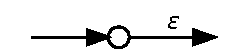
\includegraphics{parsing/basecase4}
  \caption{Fragment accepting the empty string}
  \label{fig:basecase4}
\end{figure}


%% \begin{figure}
%%   \centering
%%   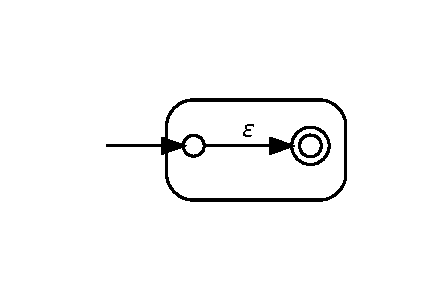
\includegraphics{parsing/basecase3}
%%   \caption{The empty string}
%%   \label{fig:basecase3}
%% \end{figure}

The first compound fragment is alternation, see figure
\vref{fig:alternation}. Here, the two sub-fragments R and S are automatons
with initial states and some dangling edges. What else they are
composed of, is irrelevant for the moment\todo{changed}. We add one new state, 
and make it the initial state for this fragment. The initial state has two
$\upvarepsilon$-edges leaving, connecting to the initial states of R
and S. The dangling edges for the new fragment is the sum of the
dangling edges leaving R and S.

\begin{figure}
  \centering
  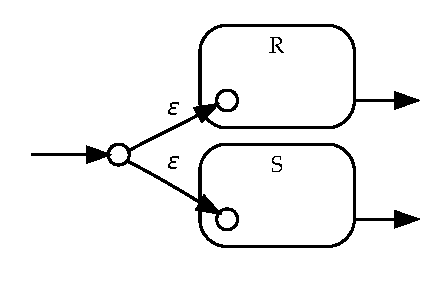
\includegraphics{parsing/alternation}
  \caption{Alternation R\textbar S}
  \label{fig:alternation}
\end{figure}

Concatenation of two regular expressions R and S is achieved as shown
in figure \vref{fig:concatenation}. The dangling edges of R is
connected to the initial state of S. The initial state for the new
fragment is the initial state of R and the dangling edges of S is
still left dangling.

\begin{figure}
  \centering
  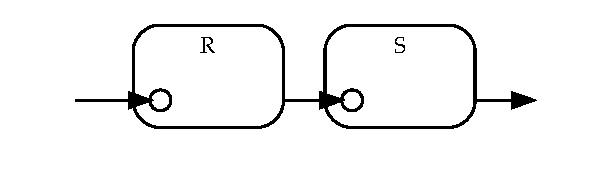
\includegraphics{parsing/concatenation}
  \caption{Concatenation RS}
  \label{fig:concatenation}
\end{figure}

Zero or more times repetition is shown in figure
\vref{fig:repetition}. One new, initial, state is added. It has two
$\upvarepsilon$-edges leaving, one is connected to the initial state of
R and one is left dangling. The dangling edges of R is connected to
the new initial state.

\begin{figure}
  \centering
  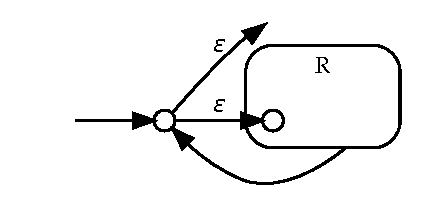
\includegraphics{parsing/repetition}
  \caption{Repetition R*}
  \label{fig:repetition}
\end{figure}

Finally an accepting state is patched into the NFA. All edges left
dangling is connected to the accepting state. 

\paragraph{Properties} NFAs created with Thompsons method has these
properties:
\begin{itemize}
  \item At most two edges is leaving a state
  \item There are no edges leaving the accepting state
  \item There are no edges leading into the starting state
\end{itemize}


\begin{example}[Converting a regular expression to a NFA]
\label{ex:converting_a_regular_expression_to_a_nfa}
\begin{figure}
  \centering 
  \subfigure[Fragment for \textsf{a}]{
    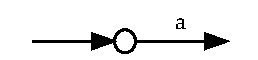
\includegraphics{parsing/ex_a.pdf}
    \label{fig:ex_parsing_a}
  }
  \subfigure[Fragment for \textsf{b}]{
    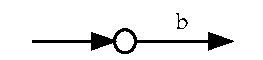
\includegraphics{parsing/ex_b.pdf}
    \label{fig:ex_parsing_b}
  }
  \subfigure[Fragment for \textsf{c}]{
    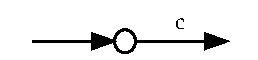
\includegraphics{parsing/ex_c.pdf}
    \label{fig:ex_parsing_c}
  }
  \subfigure[Fragment for \textsf{a*}]{
    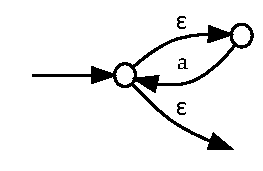
\includegraphics{parsing/ex_star.pdf}
    \label{fig:ex_parsing_star}
  }
  \subfigure[Fragment for \textsf{a*b}]{
    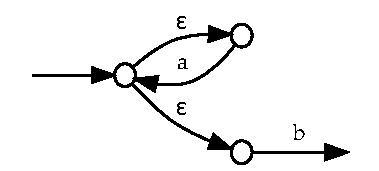
\includegraphics{parsing/ex_concat.pdf}
    \label{fig:ex_parsing_concat}
  }
  \subfigure[Fragment for \textsf{a*b\textbar c}]{
    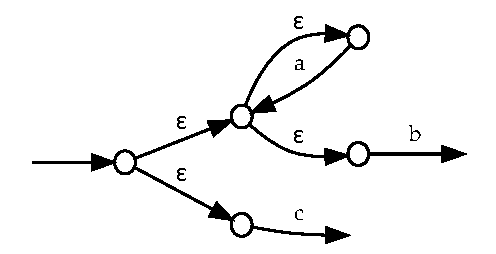
\includegraphics{parsing/ex_alt.pdf}
    \label{fig:ex_parsing_alt}
  }
  \subfigure[Final NFA for \textsf{a*b\textbar c}]{
  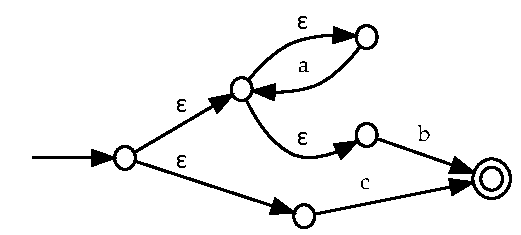
\includegraphics{parsing/ex_finished.pdf}
  \label{fig:ex_parsing_finished}
  }
  \caption{Individual fragments when converting \textsf{a*b\textbar c}
    to NFA}
  \label{fig:ex_parsing}
\end{figure}

\begin{figure}
\end{figure}


In this example we will be converting the regular expression
\textsf{a*b\textbar c} to a NFA using Thompsons method.
\begin{itemize}
\item Top level we have the alternation operator, but before we can
  complete this fragment, we need to convert \textsf{a*b} and
  \textsf{c} to fragments.
  \begin{itemize}
  \item \textsf{a*b} is complicated since we have one operator, two
    literals and a hidden concatenation. Top level we have the
    concatenation operator, concatenating \textsf{a*} and
    \textsf{b}. These needs to be converted before we can concatenate.
    \begin{itemize}
    \item \textsf{a*} needs to be broken further down. Top level we have
      the Kleene star, but we can not apply the rule for converting this
      to a NFA fragment before we have converted \textsf{a}. 
      \begin{itemize}
        \item \textsf{a} is straightforward, we just apply the rule
          for transforming literals and we have the fragment in figure
          \ref{fig:ex_parsing_a}
      \end{itemize}
      Using this fragment to complete the Kleene star, we have the
      fragment in figure \ref{fig:ex_parsing_star}.
    \item \textsf{b} is straightforward, we just apply the rule for
      transforming literals and we have the fragment in figure
      \ref{fig:ex_parsing_b}.
    \end{itemize}
    Now we are ready to concatenate, fragments
    \ref{fig:ex_parsing_star} and \ref{fig:ex_parsing_b} are
    concatenated and we have the fragment in figure \ref{fig:ex_parsing_concat}
  \item \textsf{c} is straightforward, we just apply the rule for
    transforming literals and we have the fragment in figure
    \ref{fig:ex_parsing_c}.
  \end{itemize}
  With these expressions converted to fragments we can apply the
  alternation conversion rule. We have the resulting fragment in
  figure \ref{fig:ex_parsing_alt}
\end{itemize}

All that is left now is to connect the dangling edges to an accepting
state. We have the final result in figure \vref{fig:ex_parsing_finished}
  
\end{example}

\subsection{Matching}

The NFAs constructed as described in section
\vref{sec:from_regular_expression_to_nfa} can be used to match a
regular expression with a string, i.e. to determine if a string belongs
to the language of the regular expression. 

Once the NFA is generated, simulating it is a straightforward
task. Again, our method is attributed to Thompson
\cite{Thompson1968}. 
\begin{enumerate}
    \item We maintain a set of active states and a pointer
    to the current character in the string
    \item At the beginning only the
    start state belongs to the set of active states
    \item The string is read
    from left to right, taking each character in turn. When a character is
    read from the input string, all legal transitions from the states in
    the active set is followed
    \item A transition is legal if it is a
    $\upvarepsilon$-transition or if the mark on the transition matches
    the character read from the input string. The new set of active states
    is the set of end states for the transitions followed
    \item If the
    accepting state is included in the active set when the string is read,
    the string matches the regular expression
\end{enumerate}

With this method we only ever add a state to the active set once per
iteration and we only read each character from the input string once.


\begin{example}[Matching with a NFA]
  \begin{figure}
    \centering
    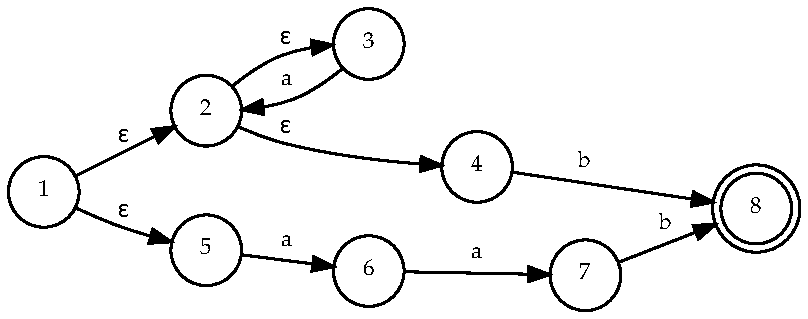
\includegraphics[width=\textwidth]{matching/ex_matching.pdf}
    \caption{NFA for the regular expression \textsf{a*b\textbar aab}}
    \label{fig:ex_matching}
  \end{figure}
  
  In this example we will demonstrate how the regular expression
  \textsf{a*b\textbar aab} is matched with the string \textsl{aab}. In
  figure \vref{fig:ex_matching} we have the corresponding NFA. Each
  state is marked with a unique number which we will be referring to
  in the table below.

\begin{center}
\begin{tabular}{ccp{8.5cm}}
Active set & \texttt{SP} & Explanation \\
\hline

1 & \textsl{\underline{a}ab} & Initially we have the start state in
the active set and \texttt{SP} points to the start of the string. \\

3, 4, 5 & \textsl{\underline{a}ab} & Following all
$\upvarepsilon$-transitions. \\

2, 6 & \textsl{a\underline{a}b} & Reading the first \textsl{a} from the input
string, states 3 and 5 have legal transitions on \textsl{a}. \\

3, 4, 6 & \textsl{a\underline{a}b} & Following all
$\upvarepsilon$-transitions. \\

2, 7 & \textsl{aa\underline{b}} & Reading the second \textsl{a} from
the input string, states 3 and 6 have legal transitions on
\textsl{a}. \\

3, 4, 6 & \textsl{aa\underline{b}} & Following all
$\upvarepsilon$-transitions. \\

8 & \textsl{aab\underline{ }} & Reading the last character from input
string: \textsl{b}, states 4 and 7 have legal transitions on
\textsl{b}. \\

8 & \textsl{aab\underline{ }} & No $\upvarepsilon$-transitions to follow.

\end{tabular}
\end{center}

After reading the string we can see that the accepting state is in the
active set: We have a match!

\end{example}



\subsection{Summary}

Regular expressions are a widely used and popular tool. The features
offered and the semantics vary. For example some will offer back
referencing and others will not, some will offer a leftmost match in
alternations, others will offer a longest match. Even for engines with
similar feature sets, the underlying implementation and performance
can vary widely. A regular expression engine can typically solve some
types of problems more efficiently than others, or vice versa: it may
be particularly bad at a given problem. %\todo{Jan: changed}

There are many highly specialized regular expression engines
exemplifying this. To briefly mention an example: Structured text like
SGML documents benefits from a different approach. Many times you will
need to find the text between two tags, but many tools are not geared
for this kind of search: The search can span several lines and we will
usually want a shortest match. See \cite{pedersen2010} for details.

To the knowledge of the writers, there is no others pursuing a regular
expression engine build on the design described in this thesis. The
division of the workload in several different components using parse
trees to communicate progress is unique. What we hope by this approach
is flexibility and a guaranteed upper bound on memory consumed for a
match.

%\todo[inline]{Might want to give an example}

%% \todo[inline]{write something about how regular expressions can be
%%   very powerful but the underlying design and its performance can vary
%% widely}



\subsection{Regular expression to NFA}
\label{sec:from_regular_expression_to_nfa}
Every regular expressions can be converted to a NFA matching the same
language.  This section will describe an approach to doing so.

\subsubsection{Thompson}
\label{sec:re2nfa_thompson_theory}
The method described in this section first appeared in Ken Thompsons
article from 1968 \cite{Thompson1968}. The descriptions given in for
example \cite{HopcroftJohnE.AndMotwaniRajeevAndUllman2001},
\cite{Aho:1986:CPT:6448} and \cite{RussCox} are considered more
readable and we will be basing our description on these.

The NFA will be build in steps from smaller NFA fragments. A NFA
fragment has an initial state, but no accepting state, instead it has
one or more dangling edges leading nowhere (yet).


%% a method for converting a
%% regular expression to an automaton is described. The method works by
%% breaking the regular expression up into fragments; Each fragment also
%% being a regular expression in itself. Using this method yields an
%% automaton with the following characteristics:
%% \begin{itemize}
%% \item There is exactly one initial state
%% \item There are no edges into the initial state
%% \item There is exatly one accepting state
%% \item There are no edges out of the accepting state
%% \item There are at most two edges leaving a state
%% \end{itemize}

The base fragment corresponds to the regular expression consisting
only of a single character \textit{a}. The NFA fragment is shown in
figure \vref{fig:basecase1}. One state with a single edge, marked with
the character \textit{a} is added. The new state is the initial state
for this fragment and the edge is left dangling.

\begin{figure}
  \centering
  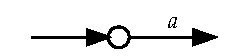
\includegraphics{parsing/basecase1}
  \caption{Fragment accepting a single character \textit{a}}
  \label{fig:basecase1}
\end{figure}

The second base fragment corresponds to the empty regular
expression. The NFA fragment is shown in figure
\vref{fig:basecase4}. One state with a single edge marked as a
$\upvarepsilon$-edge is added. The new state is the initial state for
this fragment and the edge is left dangling. This fragment is used for
the empty regular expression and for alternations with one or more
options left empty.

%% In Ken Thompson article from 1968 \cite{Thompson1968}, in
%% \cite{HopcroftJohnE.AndMotwaniRajeevAndUllman2001} and in
%% \cite{RussCox} a method for converting a regular expression to an
%% automaton is described.



%% The base case is the regular expression consisting of a single
%% character \textit{a}. Figure \vref{fig:basecase1} shows an automaton
%% accepting the same language. 

\begin{figure}
  \centering
  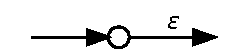
\includegraphics{parsing/basecase4}
  \caption{Fragment accepting the empty string}
  \label{fig:basecase4}
\end{figure}


%% \begin{figure}
%%   \centering
%%   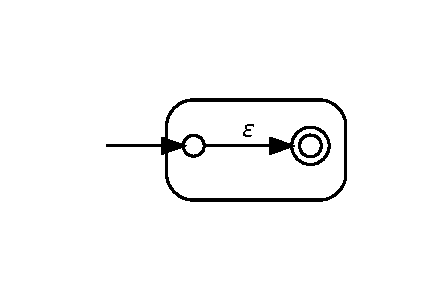
\includegraphics{parsing/basecase3}
%%   \caption{The empty string}
%%   \label{fig:basecase3}
%% \end{figure}

The first compound fragment is alternation, see figure
\vref{fig:alternation}. Here, the two sub-fragments R and S are automatons
with initial states and some dangling edges. What else they are
composed of, is irrelevant for the moment\todo{changed}. We add one new state, 
and make it the initial state for this fragment. The initial state has two
$\upvarepsilon$-edges leaving, connecting to the initial states of R
and S. The dangling edges for the new fragment is the sum of the
dangling edges leaving R and S.

\begin{figure}
  \centering
  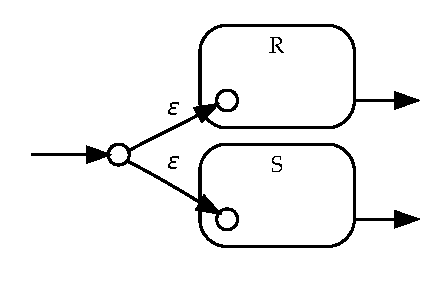
\includegraphics{parsing/alternation}
  \caption{Alternation R\textbar S}
  \label{fig:alternation}
\end{figure}

Concatenation of two regular expressions R and S is achieved as shown
in figure \vref{fig:concatenation}. The dangling edges of R is
connected to the initial state of S. The initial state for the new
fragment is the initial state of R and the dangling edges of S is
still left dangling.

\begin{figure}
  \centering
  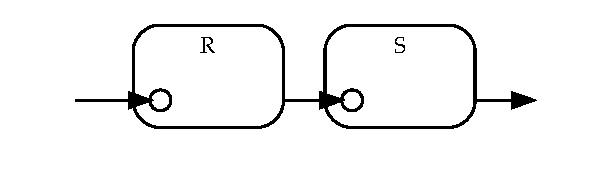
\includegraphics{parsing/concatenation}
  \caption{Concatenation RS}
  \label{fig:concatenation}
\end{figure}

Zero or more times repetition is shown in figure
\vref{fig:repetition}. One new, initial, state is added. It has two
$\upvarepsilon$-edges leaving, one is connected to the initial state of
R and one is left dangling. The dangling edges of R is connected to
the new initial state.

\begin{figure}
  \centering
  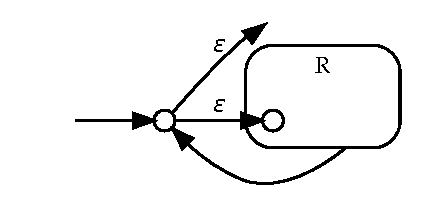
\includegraphics{parsing/repetition}
  \caption{Repetition R*}
  \label{fig:repetition}
\end{figure}

Finally an accepting state is patched into the NFA. All edges left
dangling is connected to the accepting state. 

\paragraph{Properties} NFAs created with Thompsons method has these
properties:
\begin{itemize}
  \item At most two edges is leaving a state
  \item There are no edges leaving the accepting state
  \item There are no edges leading into the starting state
\end{itemize}


\begin{example}[Converting a regular expression to a NFA]
\label{ex:converting_a_regular_expression_to_a_nfa}
\begin{figure}
  \centering 
  \subfigure[Fragment for \textsf{a}]{
    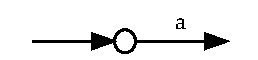
\includegraphics{parsing/ex_a.pdf}
    \label{fig:ex_parsing_a}
  }
  \subfigure[Fragment for \textsf{b}]{
    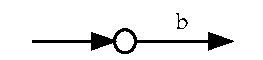
\includegraphics{parsing/ex_b.pdf}
    \label{fig:ex_parsing_b}
  }
  \subfigure[Fragment for \textsf{c}]{
    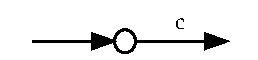
\includegraphics{parsing/ex_c.pdf}
    \label{fig:ex_parsing_c}
  }
  \subfigure[Fragment for \textsf{a*}]{
    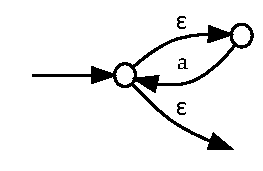
\includegraphics{parsing/ex_star.pdf}
    \label{fig:ex_parsing_star}
  }
  \subfigure[Fragment for \textsf{a*b}]{
    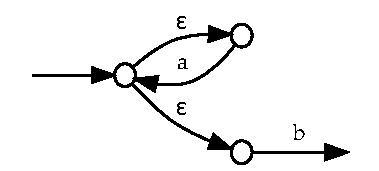
\includegraphics{parsing/ex_concat.pdf}
    \label{fig:ex_parsing_concat}
  }
  \subfigure[Fragment for \textsf{a*b\textbar c}]{
    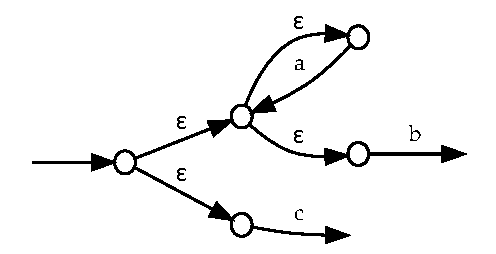
\includegraphics{parsing/ex_alt.pdf}
    \label{fig:ex_parsing_alt}
  }
  \subfigure[Final NFA for \textsf{a*b\textbar c}]{
  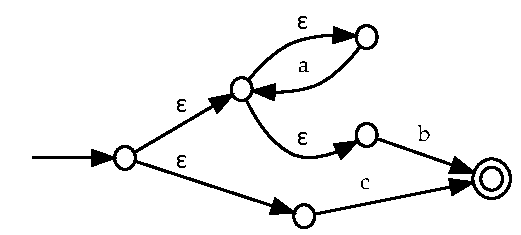
\includegraphics{parsing/ex_finished.pdf}
  \label{fig:ex_parsing_finished}
  }
  \caption{Individual fragments when converting \textsf{a*b\textbar c}
    to NFA}
  \label{fig:ex_parsing}
\end{figure}

\begin{figure}
\end{figure}


In this example we will be converting the regular expression
\textsf{a*b\textbar c} to a NFA using Thompsons method.
\begin{itemize}
\item Top level we have the alternation operator, but before we can
  complete this fragment, we need to convert \textsf{a*b} and
  \textsf{c} to fragments.
  \begin{itemize}
  \item \textsf{a*b} is complicated since we have one operator, two
    literals and a hidden concatenation. Top level we have the
    concatenation operator, concatenating \textsf{a*} and
    \textsf{b}. These needs to be converted before we can concatenate.
    \begin{itemize}
    \item \textsf{a*} needs to be broken further down. Top level we have
      the Kleene star, but we can not apply the rule for converting this
      to a NFA fragment before we have converted \textsf{a}. 
      \begin{itemize}
        \item \textsf{a} is straightforward, we just apply the rule
          for transforming literals and we have the fragment in figure
          \ref{fig:ex_parsing_a}
      \end{itemize}
      Using this fragment to complete the Kleene star, we have the
      fragment in figure \ref{fig:ex_parsing_star}.
    \item \textsf{b} is straightforward, we just apply the rule for
      transforming literals and we have the fragment in figure
      \ref{fig:ex_parsing_b}.
    \end{itemize}
    Now we are ready to concatenate, fragments
    \ref{fig:ex_parsing_star} and \ref{fig:ex_parsing_b} are
    concatenated and we have the fragment in figure \ref{fig:ex_parsing_concat}
  \item \textsf{c} is straightforward, we just apply the rule for
    transforming literals and we have the fragment in figure
    \ref{fig:ex_parsing_c}.
  \end{itemize}
  With these expressions converted to fragments we can apply the
  alternation conversion rule. We have the resulting fragment in
  figure \ref{fig:ex_parsing_alt}
\end{itemize}

All that is left now is to connect the dangling edges to an accepting
state. We have the final result in figure \vref{fig:ex_parsing_finished}
  
\end{example}

\subsection{Matching}

The NFAs constructed as described in section
\vref{sec:from_regular_expression_to_nfa} can be used to match a
regular expression with a string, i.e. to determine if a string belongs
to the language of the regular expression. 

Once the NFA is generated, simulating it is a straightforward
task. Again, our method is attributed to Thompson
\cite{Thompson1968}. 
\begin{enumerate}
    \item We maintain a set of active states and a pointer
    to the current character in the string
    \item At the beginning only the
    start state belongs to the set of active states
    \item The string is read
    from left to right, taking each character in turn. When a character is
    read from the input string, all legal transitions from the states in
    the active set is followed
    \item A transition is legal if it is a
    $\upvarepsilon$-transition or if the mark on the transition matches
    the character read from the input string. The new set of active states
    is the set of end states for the transitions followed
    \item If the
    accepting state is included in the active set when the string is read,
    the string matches the regular expression
\end{enumerate}

With this method we only ever add a state to the active set once per
iteration and we only read each character from the input string once.


\begin{example}[Matching with a NFA]
  \begin{figure}
    \centering
    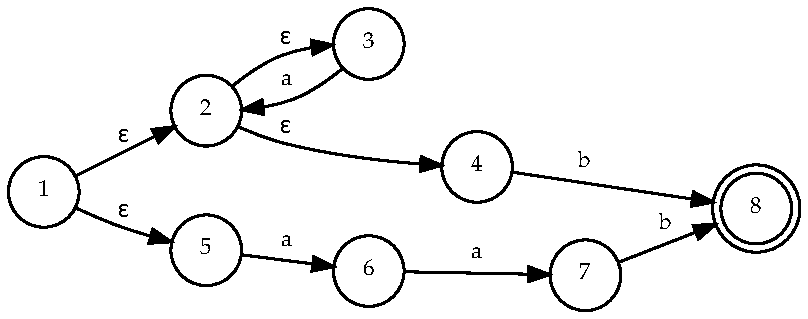
\includegraphics[width=\textwidth]{matching/ex_matching.pdf}
    \caption{NFA for the regular expression \textsf{a*b\textbar aab}}
    \label{fig:ex_matching}
  \end{figure}
  
  In this example we will demonstrate how the regular expression
  \textsf{a*b\textbar aab} is matched with the string \textsl{aab}. In
  figure \vref{fig:ex_matching} we have the corresponding NFA. Each
  state is marked with a unique number which we will be referring to
  in the table below.

\begin{center}
\begin{tabular}{ccp{8.5cm}}
Active set & \texttt{SP} & Explanation \\
\hline

1 & \textsl{\underline{a}ab} & Initially we have the start state in
the active set and \texttt{SP} points to the start of the string. \\

3, 4, 5 & \textsl{\underline{a}ab} & Following all
$\upvarepsilon$-transitions. \\

2, 6 & \textsl{a\underline{a}b} & Reading the first \textsl{a} from the input
string, states 3 and 5 have legal transitions on \textsl{a}. \\

3, 4, 6 & \textsl{a\underline{a}b} & Following all
$\upvarepsilon$-transitions. \\

2, 7 & \textsl{aa\underline{b}} & Reading the second \textsl{a} from
the input string, states 3 and 6 have legal transitions on
\textsl{a}. \\

3, 4, 6 & \textsl{aa\underline{b}} & Following all
$\upvarepsilon$-transitions. \\

8 & \textsl{aab\underline{ }} & Reading the last character from input
string: \textsl{b}, states 4 and 7 have legal transitions on
\textsl{b}. \\

8 & \textsl{aab\underline{ }} & No $\upvarepsilon$-transitions to follow.

\end{tabular}
\end{center}

After reading the string we can see that the accepting state is in the
active set: We have a match!

\end{example}



\section{Matching}

The NFAs constructed as described in section
\vref{sec:from_regular_expression_to_nfa} can be used to match a
regular expression with a string, i.e. to decide if a string belongs
to the language of the regular expression. 


Once the NFA is generated, simulating it is a straightforward task. We
maintain a set of active states and a pointer to the current character
in the string. At the beginning only the start state belongs to the
set of active states. The string is read from left to right, taking
each character in turn. When a character is read from the input
string, all legal transitions from the states in the active set is
followed. A transition is legal if it is a $\upvarepsilon$-transition
or if the mark on the transition matches the character read from the
input string. The new set of active states is the set of end states
for the transitions followed. If the accepting state is included in
the active set when the string is read, the string matches the regular
expression.

With this method we only ever add a state to the active set once per
iteration and we only read each character from the input string once.


\begin{example}[Matching with a NFA]
  \begin{figure}
    \centering
    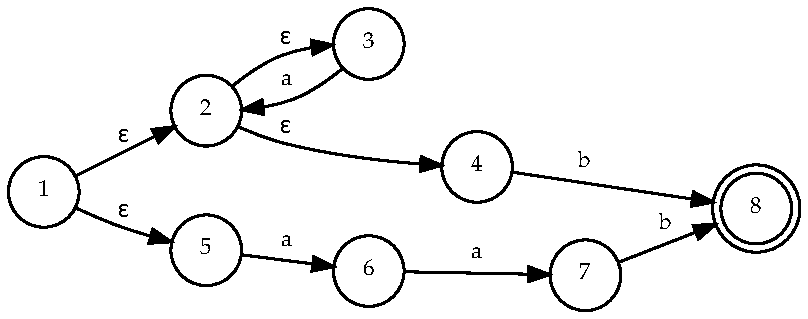
\includegraphics[width=\textwidth]{matching/ex_matching.pdf}
    \caption{NFA for the regular expression \textsf{a*b\textbar aab}}
    \label{fig:ex_matching}
  \end{figure}
  
  In this example we will demonstrate how the regular expression
  \textsf{a*b\textbar aab} is matched with the string \textsl{aab}. In
  figure \vref{fig:ex_matching} we have the corresponding NFA. Each
  state is marked with a unique number which we will be referring to
  in the table below.

\begin{center}
\begin{tabular}{ccp{8.5cm}}
Active set & \texttt{SP} & Explanation \\
\hline

1 & \textsl{\underline{a}ab} & Initially we have the start state in
the active set and \texttt{SP} points to the start of the string. \\

3, 4, 5 & \textsl{\underline{a}ab} & Following all
$\upvarepsilon$-transitions. \\

2, 6 & \textsl{a\underline{a}b} & Reading the first \textsl{a} from the input
string, states 3 and 5 have legal transitions on \textsl{a}. \\

3, 4, 6 & \textsl{a\underline{a}b} & Following all
$\upvarepsilon$-transitions. \\

2, 7 & \textsl{aa\underline{b}} & Reading the second \textsl{a} from
the input string, states 3 and 6 have legal transitions on
\textsl{a}. \\

3, 4, 6 & \textsl{aa\underline{b}} & Following all
$\upvarepsilon$-transitions. \\

8 & \textsl{aab\underline{ }} & Reading the last character from input
string: \textsl{b}, states 4 and 7 have legal transitions on
\textsl{b}. \\

8 & \textsl{aab\underline{ }} & No $\upvarepsilon$-transitions to follow.

\end{tabular}
\end{center}

After reading the string we can see that the accepting state is in the
active set: We have a match!

\end{example}


\subsection{Protocol specification}
\label{sec:protocol_spec}

In this section we will define a protocol that can communicate
information between our processes. The information consists of the
mixed bit-values generated by the NFA simulator and the filters. The
protocol should enable us to recreate paths taken through an NFA. To
this purpose we need the protocol to support the following operators:

\begin{description}
  \item[\textbar] The end of the channel list is reached and we should
    set the active channel to the first channel. This coincides with
    reading a new character. It is not a strictly necessary operator,
    we can make do with the change channels action. We choose to keep
    a separate action for end of list, because it adds to readability
    and redundancy.
  \item[:] Whenever we change channels we put a :. There may be more
    than one or perhaps even no bits output on a channel for any given
    character from the string
  \item[=] Copying of a channel. One channel is split into two, the
    paths taken through the NFA will be identical up to the point of
    splitting. The newly created channel is put in front of the rest
    of the channels
  \item[0,1, \textbackslash $a$] The actual bit values. The character
    classes needs extra care, we need to know on which character we
    passed them, so we put the value we pass on, escaped in the output
  \item[b] A channel is abandoned with no match
  \item[t] A channel has a match
\end{description}

\begin{example}[Protocol]
  In figure \vref{fig:ex_prot} we have an automaton for regular
  expression \textsf{a*}. When matching this regular expression with
  the string \textsl{aa} we generate some mixed bit-values. This
  example will in detail demonstrate how the mixed bit-values are
  generated.
  \begin{figure}
    \centering
    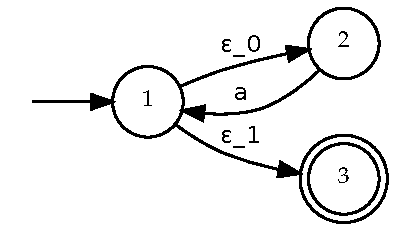
\includegraphics{matching/example_protocol.pdf}
    \caption{Automaton with bitvalues for regular expression
      \texttt{a*}}
    \label{fig:ex_prot}
  \end{figure}
  
  \begin{description}
  
  \item[Initial step:] Initially the start state of the automaton is
    added to the active list. All $\upvarepsilon$-edges are followed
    and the following is output:
    \begin{enumerate}
    \item Node 1 is a split-node, a \texttt{=} is output, and we
      follow the $\upvarepsilon$-edge to node 2 and output a
      \texttt{0}. We can not make any further progress on this
      channel. We output a \texttt{:} and switch to the next channel.

      Output so far: \texttt{=0:}. \\
      List of active channels: $\{2, 1\}$.
    \item The active channel is now in node 1, we follow the
      $\upvarepsilon$-edge from node 1 to 3 and output a
      \texttt{1}. We can not make any further progress on this
      channel. This is the last channel in the channel list, so we
      output a \texttt{|} and reset the active channel.

      Output so far: \texttt{=0:1|}.\\
      List of active channels: $\{2, 3\}$.
    \end{enumerate}

  \item[First \textsl{a} is read]
    \begin{enumerate}
    \item Node 2 has a transition marked \texttt{a}, we follow this
      back to node 1. Node 1 is a split-node, a \texttt{=} is output,
      and we follow the $\upvarepsilon$-edge to node 2 and output a
      \texttt{0}. We can not make any further progress on this
      channel. We output a \texttt{:} and switch to the next channel.

      Output so far: \texttt{=0:1|=0:}. \\
      List of active channels: $\{2, 1, 3\}$.
    \item The active channel is now in node 1, we follow the
      $\upvarepsilon$-edge from node 1 to 3 and output a
      \texttt{1}. We can not make any further progress on this
      channel. We output a \texttt{:} and switch to the next channel.

      Output so far: \texttt{=0:1|=0:1:}. \\
      List of active channels: $\{2, 3, 3\}$.
    \item Node 3 is the accepting node and does not have any
      transitions. We abandon this channel and output a
      \texttt{b}. This is the last channel in the channel list, so we
      output a \texttt{|} and reset the active channel.

      Output so far: \texttt{=0:1|=0:1:b|}. \\
      List of active channels: $\{2, 3\}$.
    \end{enumerate}
  \item[Second \textsl{a} is read] This is the final step.
    \begin{enumerate}
      \item From node 2 we can make a transition on \texttt{a} back to
        node 1. This is a split node, so we output a \texttt{=} and
        transition on the the $\upvarepsilon$-edge to node 2 and
        output a \texttt{0}. We can not do further transitions and
        this is not the accepting node, we abandon this channel and
        output a \texttt{b}. We switch to the next channel and output
        a \texttt{:}.

        Output so far: \texttt{=0:1|=0:1:b|=0b:}. \\
        List of active channels: $\{1, 3\}$.
      \item Node 1 has a $\upvarepsilon$-transition to node 3, we take
        it and output a \texttt{1}. We can not do further transitions
        and since this is the accepting node, we output a
        \texttt{t}. We have one channel left, so we output a
        \texttt{:} and switch.

        Output so far: \texttt{=0:1|=0:1:b|=0b:1t:}. \\
        List of active channels: $\{3\}$.
      \item Node 3 has no available transitions. We abandon this
        channel and output a \texttt{b}.

        Output so far: \texttt{=0:1|=0:1:b|=0b:1t:b}. \\
        List of active channels: $\{\}$.
    \end{enumerate}
  \end{description}
\end{example}



\subsection{Filters}

We have now established that filters are stand-alone programs that
takes input, performs some projection and outputs the result. In this
subsection we will give a more detailed description of the filters
developed for this thesis. 

The filters can be combined to make a whole, naturally some orders of
combining makes more sense than others. For example will it make sense
to have filters removing unnecessary information as early as possible,
to reduce the input data-sizes for downstream filters.

%% \todo[inline]{Better introduction or consider merging with architecture}

%% \todo[inline]{Describe orders of filters}


\subsubsection{The 'match' filter}

\paragraph{Input} Any mixed bit-values or bit-values
\paragraph{Output} A single value indicating match or no match.
\paragraph{}

This is a simple filter. The input is scanned for a \texttt{t} control
character, if present we output a \texttt{t} otherwise we output a
\texttt{b}. In the case of empty input, we will output an error
message, this is because the empty input is most likely due to an
error in the previous programs. To save time on processing, we will
assume the input format is correct.

\begin{example}
The regular expression \textsf{a*} matches the string \textsl{aaa}:
\begin{verbatim}
$ echo -n 'aaa' | ./main 'a*' | ./ismatch 
t
\end{verbatim}
\textsf{a*} does \emph{not} match \textsl{bbb}:
\begin{verbatim}
$ echo -n 'bbb' | ./main  'a*' | ./ismatch 
b
\end{verbatim}
Since we do not check the correctness of the input, the sentence:
``the cake is a lie'' which is clearly not in the correct input format
with regards to the protocol defined section \vref{sec:protocol_spec},
will also produce a positive answer from the filter:
\begin{verbatim}
$ echo -n 'the cake is a lie' | ./ismatch
t
\end{verbatim}

\end{example}

\subsubsection{The 'trace' filter}
\label{sec:desc_materialize}
\paragraph{Input} Mixed bit-values
\paragraph{Output} Bit-values
\paragraph{}

The mixed bit-values is a way of keeping track of multiple paths
through the NFA. This filter will remove all channels from the mixed
bit-values, except the one that has a match. We are using
Thompsons method for matching, so we can be sure there is at most one
channel with a match. 

This will be a non-streaming filter. This problem can not be solved
without in some way storing the mixed bit-values: We need knowledge of
whether or not a channel has a match at the beginning, but we will not
have that knowledge until the end.

\begin{example}
In the previous example we saw that the regular expression \textsf{a*}
matches the string \textsl{aaa}. The NFA for the regular expression is
in figure \vref{fig:ex_prot}, marked with state numbers and
bit-values. This particular match will generate the following mixed
bit-values: \texttt{=0:1|=0:1:b|=0:1:b|=0b:1t:b}. The filter should
then only return the bit-values \texttt{0001}, which represents the
match. The filter should return the empty string if there is no match.
\end{example}


\subsubsection{The 'groupings' filter}
\label{sec:groupings_filter_analysis}
\paragraph{Input} Mixed bit-values
\paragraph{Output} Mixed bit-values for rewritten regular expression
\paragraph{}

This filter facilitates reporting the content of captured groups. The
filter outputs the mixed bit-values associated with the groupings. By
this we mean that all mixed bit-values generated while inside a
captured group should be sent to output and all mixed bit-values
generated outside a group should be thrown away. By throwing away the
unnecessary bit-values we hope to make the mixed bit-values sequence
shorter. This will be an advantage when the time comes to apply the
trace filter, which is non-streaming, described in section
\vref{sec:desc_materialize}.

\begin{example}[Simple groupings filter]
  \label{ex:simple_groupings}
  Here we have a few simple examples of what the groupings filter
  should do. 
  \begin{itemize}
  \item
    For regular expression \textsf{(a\textbar b)} matched with
    \textsl{a} the mixed bit-values are \texttt{=0:1\textbar t:b}. Since
    the whole regular expression is contained in a capturing
    parenthesis, nothing should be thrown away. Output should contain
    \texttt{=0:1\textbar t:b}.
  \item
    For regular expression \textsf{(?:a\textbar b)(c\textbar d)} matched
    with \textsl{ac} the mixed bit-values are
    \texttt{=0:1|=0:1:b|t:b}. This time the first part of the regular
    expression is contained only in a non-capturing parenthesis and the
    associated bit-values should be thrown away. We want to keep only the
    bit-values from the second alternation. Output should contain
    \texttt{=:|=0:1:b|t:b}.
  \end{itemize}
  
  In this example we have only dealt with simple examples. Regular
  expressions containing parenthesis under alternation and repetition,
  e.g. \textsf{(a)\textbar b} and \textsf{(a)*}, require extra care
  and will be discussed later.
\end{example}

The output of the groupings filter can be used to navigate the NFA for
the regular expression altered in a similar manner: Everything not in
a capturing parenthesis is thrown away. From example
\vref{ex:simple_groupings} we have the regular expression
\textsf{(?:a\textbar b)(c\textbar d)}, if we throw away everything not
in a capturing parenthesis we have left \textsf{(c\textbar d)}. Stated
in a more formal manner, we can define our first naive rewriting
function $G'$:

\begin{align}
  G'[[\upvarepsilon]] &= \upvarepsilon \notag\\
  G'[[a]] &= \upvarepsilon \notag\\
  G'[[ [...] ]] &= \upvarepsilon \notag\\
  G'[[r'r_2]] &= G'[[r']]G'[[r_2]] \notag\\
  G'[[r'|r_2]] &= G'[[r']]G'[[r_2]] \notag\\
  G'[[r*]] &= G'[[r]] \notag\\
  G'[[r+]] &= G'[[r]] \notag\\
  G'[[r?]] &= G'[[r]] \notag\\
  G'[[(?:r)]] &= G'[[r]] \label{eq:G1_paren}\\
  G'[[(r)]] &= (r) \notag
\end{align}

\paragraph{Capturing under alternation}
As is seen, $G'$ basically throws away anything not in a capturing
parenthesis. There are however a few problems with this definition, as
hinted earlier. Our first problem is regular expression with a
capturing parenthesis under alternation. When the capturing
parenthesis is under the alternation and we throw away the
alternation, we lose a vital choice: There is no longer a way to
signal whether or not a group participates in a match.
\begin{figure}
  \centering
  \subfigure[\textsf{(a)\textbar (b)}]{
    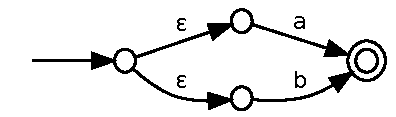
\includegraphics{filters/capturing_under_parenthesis1.pdf}
    \label{fig:capt_paren1}
  }
  \subfigure[\textsf{(a)(b)}]{
    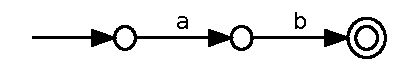
\includegraphics{filters/capturing_under_parenthesis2.pdf}
    \label{fig:capt_paren2}
  }
  \subfigure[\textsf{(?:\textbar (a))(?:\textbar (b))}]{
    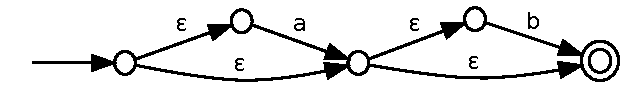
\includegraphics{filters/capturing_under_parenthesis3.pdf}
    \label{fig:capt_paren3}
  }
\caption{Capturing under alternation}
\end{figure}

\begin{example}[Capturing under alternation]
  \label{ex:capturing_under_alternation}
  In matching the regular expression \textsf{(a)\textbar (b)}, see
  figure \vref{fig:capt_paren1} for the NFA, with the string
  \textsl{a} we obtain these mixed bit-values: 
  \begin{center}\texttt{=0:1|t:b}\end{center}
  What these mixed bit-values are saying is that we have 2 channels,
  one that go through \textsf{a} and succeeds and one that go through
  \textsf{b} and fails. The succeeding channel never goes through
  \textsf{b}, the contents of that group is not defined.
  
  Rewriting the regular expression \textsf{(a)\textbar (b)} according
  to $G'$ we have:
  \begin{align*}
    G'[[\text{\textsf{(a)\textbar (b)}}]] &=
    G'[[\text{\textsf{(a)}}]]G'[[\text{\textsf{(b)}}]] \\
    &= \text{\textsf{(a)}}\text{\textsf{(b)}} \\
  \end{align*}
  In this regular expression there is only one way: The one going
  through both the groups. See figure \vref{fig:capt_paren2} for the
  NFA of the expression. This is bad news for our rewriting function
  and our filter, since we need some way of skipping groups: Each
  channel goes through only one group.
\end{example}

In example \ref{ex:capturing_under_alternation} we saw an example of
how undefined groups are not handled. To solve this problem we need
some way of signaling if a group participates in a match or not. We
define a new rewriting function $G''$ it is identical to $G'$ except
for equation \ref{eq:G1_paren} which is changed to:
\begin{align}
    G''[[(r)]] &= (?:|(r)) \notag
\end{align}
This change will enable us to choose which groups participates in a
match. This comes at a cost: Extra bits will have to be added to the
mixed bit-values output and extra alternations to the rewritten
regular expression. 

\begin{example}[continues=ex:capturing_under_alternation]
With the changed equation \ref{eq:G1_paren} we can continue our
example from before. Again we rewrite regular expression
\textsf{(a)\textbar (b)}, this time according to $G''$:
  \begin{align*}
    G''[[\text{\textsf{(a)\textbar (b)}}]] &=
    G''[[\text{\textsf{(a)}}]]G''[[\text{\textsf{(b)}}]] \\
    &= \text{\textsf{(?:\textbar (a))(?:\textbar (b))}} \\
  \end{align*}
  See figure \vref{fig:capt_paren3} for the NFA. As is clear from the
  rewritten regular expression and the NFA, there is now a way around
  the groups. Taking this into account, the output for the groupings
  filter should be: 
  \begin{center}\texttt{=1:01|0t:b}\end{center}
  What these mixed bit-values are saying is that we have two channels,
  one picks the route through \textsf{a}, around \textsf{b} and
  succeeds and the other picks the route around \textsf{a}, through
  \textsf{b} and fails.
\end{example}
As needed, we now have a way of signaling if a particular group is in
a match: Insert a 1 in the mixed bit-values and the group participates
or insert a 0 and it does not. 


\paragraph{Capturing under repetition}
The other problem we hinted at has to do with capturing under
repetition. When using a capturing subpattern, it can match repeatedly
using a quantifier. For example matching \textsf{(.)*} with the string
\textsl{abc}, the first time we apply the \textsf{*} we capture a
\textsl{a} the second time a \textsl{b} and the last time a
\textsl{c}. In such a case we have several options when reporting the
strings that was captured:
\begin{itemize}
\item The first
\item The last, this is the what most backtracking engines like Perl
  do
\item All, this is what a full regular expression engine do
\end{itemize}
Only two of these options are available to a streaming filter: All and
the first. In order to return the last match, we would have to save
the latest match when matching with the quantifier, it is potentially
the last and we can not know until we are done matching with the
quantifier.

Returning the first string that was captured by the quantifier, forces
us to throw away mixed bit-values generated in a capturing
parenthesis. We would only need the mixed bit-values generated by the
first iteration of the quantifier. 

To return all the strings captured by a group, we simply output all
the mixed bit-values generated while in the capturing
parenthesis. However, this causes problems with the rewriting
function. Rewriting \textsf{(.)*} according to $G''$ we have
\textsf{(.)}. This regular expression accepts one single character. In
no way can we make mixed bit-values, fitting this regular expression,
that represent a list of matched strings. Therefore we add the
following equations:
\begin{align*}
  G''[[(r)*]] &= (r)* \\
  G''[[(r)+]] &= (r)+
\end{align*}
We should now also keep the mixed bit-values that glues the iterations
together, even though they are outside the capturing group.




%% \begin{example}[Capturing under repetition]
%%   %% \begin{figure}
%%   %%   \centering
%%   %%   \subfigure[\textsf{(a)*}]{
%%   %%     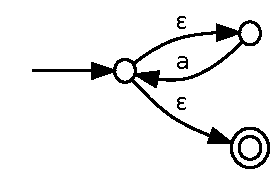
\includegraphics{filters/capt_under_rep1.pdf}
%%   %%     \label{fig:capt_rep1}
%%   %%   }
%%   %%   \subfigure[\textsf{(a)}]{
%%   %%     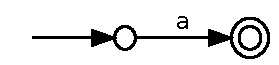
\includegraphics{filters/capt_under_rep2.pdf}
%%   %%     \label{fig:capt_rep2}
%%   %%   }
%%   %%   \caption{Capturing under repetition}
%%   %% \end{figure}

%%   %% In this example we will be matching regular expression
%%   %% \textsf{(a)*}, see figure \vref{fig:capt_rep1} for the NFA, with the
%%   %% string \textsl{aaa}. This match generates the following mixed
%%   %% bit-values:
%%   %% \begin{center}\texttt{=0:1|=0:1:b|=0:1:b|=0b:1t:b}\end{center}

%%   %% Rewriting \textsf{(a)*} according to $G''$ gives us:
%%   %% \begin{align*}
%%   %%   G''[[\text{\textsf{(a)*}}]] &= G''[[\text{\textsf{(a)}}]] \\
%%   %%   &= \text{\textsf{(a)}}
%%   %% \end{align*}
%%   %% See figure \vref{fig:capt_rep2} for the NFA.

%%   %% This rewrite works if we are only interested in one 

%%   By matching
%% \end{example}


%% To return all we need to make some changes to the rewriting function,
%% we add the following equations:
%% \begin{align*}
%%   G''[[(r)*]] &= (r)* \\
%%   G''[[(r)+]] &= (r)+
%% \end{align*}


%% We should not just throw away everything

%% If we choose to return all, all we need to do is add equations to the
%% rewriting function:
%% \begin{align*}
%%   G''[[(r)*]] &= (r)* \\
%%   G''[[(r)+]] &= (r)+
%% \end{align*}



%% Returning all would be the easier solution. We need to be careful when
%% rewriting the regular expression however. With the output from the
%% groupings filter we should be able to navigate the NFA for the
%% rewritten regular expression.


%% Returning all would be the easiest solution, this would however
%% require a change in the rewriting function. We add the equations:
%% \begin{align*}
%%   G''[[(r)*]] &= (r)* \\
%%   G''[[(r)+]] &= (r)+
%% \end{align*}


%% %% Returning all of the strings that were captured is by far the easiest,
%% %% no extra work is required. On the other hand if we only want to return
%% %% the first of the matches, we need to know whether or not to return a
%% %% particular match, that is if this is the first time we match with the
%% %% quantifier or not. If we alter the way we construct the NFA, we can
%% %% achieve this. 





%% \todo{Hvad den blippen er det nu for en løsning jeg har på det
%%   problemos}



We are now ready to present the final rewriting function: Definition
\vref{def:G}.
\begin{definition}[The groupings filter rewriting function]
  \label{def:G}
  For regular expressions $r$, $r_1$, $r_2$, defined over alphabet
  $\Sigma$, and $a$, any character from $\Sigma$, let $G$ be defined by:
  \begin{align*}
    G[[\upvarepsilon]] &= \upvarepsilon \\
    G[[a]] &= \upvarepsilon \\
    G[[ [...] ]] &= \upvarepsilon \\
    G[[r_1r_2]] &= G[[r_1]]G[[r_2]] \\
    G[[r_1|r_2]] &= G[[r_1]]G[[r_2]] \\
    G[[r*]] &= G[[r]] \\
    G[[r+]] &= G[[r]] \\
    G[[r?]] &= G[[r]] \\
    G[[(?:r)]] &= G[[r]] \\
    G[[(r)]] &= (?:|(E)) \\
    G[[(r)*]] &= (?:|(r)*) \\
    G[[(r)+]] &= (?:|(r)+) \\
  \end{align*}
\end{definition}
\begin{example}
  Here follows a few examples of how the groupings filter rewriting
  function, $G$, works.
  \begin{align*}
    G[[\mathsf{(a)|b}]] &= G[[\mathsf{(a)}]]G[[\mathsf{b}]]\\
    &= \mathsf{(?:(a))} \upvarepsilon\\
    &= \mathsf{(?:(a))}
  \end{align*}

  \begin{align*}
    G[[\mathsf{((cup)cake)}]] &= \mathsf{(?:|((cup)cake))}
  \end{align*}

  \begin{align*}
    G[[\mathsf{(a|b)*}]] &= \mathsf{(a|b)*}
  \end{align*}
\end{example}



\section{Implementing a regular expression engine}
\label{sec:implementation}
The task of implementing a regular expression engine can be undertaken
in steps. The first steps is converting the regular expression to a
NFA. The next step is to simulate the NFA. The last step in our
implementation is to build filters.

%% \subsection{Datastructures}

%% \subsubsection{Representing the NFA}

%% For the representation of the NFA we started out as Russ Cox in
%% \cite{RussCox}. The NFA is represented as a linked collection of
%% \lstinline{State} structures:
%% \begin{lstlisting}
%% struct State
%% {
%%     unsigned int c;
%%     unsigned int type;
%%     struct State *out0;
%%     struct State *out1;
%% };
%% \end{lstlisting}
%% This is the essential contents of the \lstinline{State} structure. It
%% actually contains more variables, these will be added and explained
%% when appropriate. There is no explicit representation of the
%% transitions, they are represented as the two \lstinline{out} pointers in
%% the \lstinline{State} structure. The \lstinline{type}-variable decides the
%% type of the state and the transition(s):
%% \begin{description}
%% \item[split] This state is a split-state, both the two
%%   \lstinline{out}-pointers will be set to valid states.
%% \item[accepting] This is the accepting state.
%% \item[literal] This state only has a valid transition on the
%%   \lstinline{out0}-pointer. It is marked with the value in \lstinline{c}
%% \item[range] This is a state with a range-transition. These will
%%   be explained later in \vref{sec:ranges_impl}.
%% \item[epsilon] The transition in \lstinline{out0} is a
%%   $\upvarepsilon$-transition.
%% \end{description}

\subsubsection{Character classes}
\label{sec:ranges_impl}

\begin{figure}
  \centering 
  \subfigure[\textsf{[a-c]}]{
    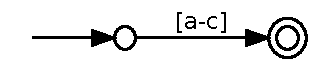
\includegraphics{implementation/range1.pdf}
    \label{fig:range1}
  }
  \subfigure[\textsf{a\textbar b\textbar c}]{
    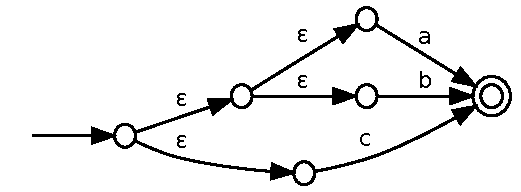
\includegraphics{implementation/range2.pdf}
    \label{fig:range2}
  }
  \caption{A simple character class-transition example}
  \label{fig:ranges}
\end{figure}

Character classes are part of the extension we made to the regular
expression definition. When implementing, we have the choice of
rewriting character classes in terms of the original regular
expressions, but as we can see in figure \vref{fig:ranges}, this
quickly becomes unwieldy. When we rewrite we add almost two states per
character matched by the character class, instead of adding just one
state for the whole character class. What we want is a NFA similar to
figure \ref{fig:range1}, not figure \ref{fig:range2}.

There are several ways of obtaining this goal. Perl uses a bitmap to
indicate membership of a range, for each character in the character
set there is a bit in the bitmap. To decide membership the bit
corresponding to the character is looked up. RE2 uses a balanced
binary tree, each node in the tree corresponds to either a whole range
or a literal character, the tree is then searched when deciding
membership. Each method has its advantages and drawbacks. The bitmap
is of constant size, so for small character classes, it will be
unnecessarily large, but the time to look up a value in the bitmap is
also constant and very fast. The balanced binary tree, has its
advantages for character classes with few ranges and literal
characters, since it will then be small in size and look up times. The
drawbacks are of course that it grows in size and look up times with
the character class.

For this project an even simpler solution was chosen: A simple linked
list of ranges. The literal characters will be represented as ranges
of length one. On other words, we will have one linked list per
character class, and the number of elements in each linked list is the
number of literals and ranges in the character class. Worst case we
will have to look through all members of a linked list to decide
membership of a character class. This is simplistic, but sufficient.

%% There should not be any serious
%% performance issues for simple character classes with few ranges and
%% literal characters.
%% \begin{lstlisting}
%% struct Range 
%% {
%%   unsigned int lo;
%%   unsigned int hi;
%%   struct Range *next;
%% };
%% \end{lstlisting}
%% The two unsigned integers are used to store the beginning and end of
%% the range, in the case of a single literal they are the same. The
%% \lstinline{next}-pointer points to the next range in the list. A
%% \lstinline{Range}-pointer and a flag to indicate whether or not the
%% character class is negated is added to the \lstinline{State} struct.

\subsection{Regular expression to NFA}

The first step in our regular expression engine is the regular
expression to NFA converter. As discussed in section
\vref{sec:re2nfa_thompson_theory}, the NFA is built from the regular
expression in steps from smaller NFA fragments. In order for this
method, used directly, to be successful, the regular expression has to
be in a form where the meta characters and the literals are presented
in the right order. Regular expressions with for example
\textsf{\textbar} can not simply be read from left to right and be
converted correctly. The problem with the alternation operator is that
it is an infix operator, so we only have the left hand side and not
the right hand side when we read the \textsf{\textbar} and can
therefore not complete the fragment.

Converting the regular expression to reverse polish notation, with an
explicit concatenation operator, or making a parse tree will solve
these problems. For this project neither is chosen. A third solution
to this problem is maintaining a stack where fragments and operators
are pushed and popped. This is the method that is implemented. We
tried determining the quality of the decision by comparing run times
with Russ Cox's example code \cite{Cox2007}. This did not go well due
to several reasons. The main reason is that the example code does not
do well on large examples\footnote{There are constants in the source
  code and a naive list append function} and large examples is needed
to do a reasonable comparison.

We followed Russ Cox' method from \cite{RussCox}, when converting the
regular expression to NFA. Russ Cox rewrites the regular expression to
reverse polish notation with an explicit concatenation operator, so
some changes will be necessary. There are tree main areas that needs
to be changed:

\begin{description}
\item[Concatenation] While constructing the NFA, NFA fragments are
  pushed onto a stack. Whenever the concatenation operator is
  encountered, the two top fragments are popped and patched together,
  see figure \vref{fig:concatenation}. We do not have the advantage of
  an explicit concatenation operator. Instead we will be trying to pop
  the top two NFA fragments and patching them together as often as
  possible. As often as possible is after a character is read, but
  before any action is taken on the character read. The exception to
  this rule is the quantifiers, which binds tighter than
  concatenation.
\item[Parentheses] The binding of the operators can be changed with
  parentheses. Not using a tree structure or reverse polish notation
  with an explicit concatenation operator, there is nothing showing
  the structure of how everything binds when simply reading the
  regular expression from left to right. We need some way of
  connecting the left parentheses to the matching right
  parentheses. For this we will be using the stack, we will expand it
  to also accept operators. Every time we read a left parenthesis in
  the regular expression, a left-parenthesis-fragment is pushed onto
  the stack. When we later on read a right parenthesis we simply pop
  fragments of the stack and patch them together till we reach a
  left-parenthesis-fragment.   
\item[Alternation] When reading the regular expression left to right,
  we only have the left NFA fragment ready when reading the
  alternation operator. Therefore we simply push the alternation
  operator on the stack. Whenever possible we pop the alternation
  operator and associated NFA fragments and patch them together, see
  figure \vref{fig:alternation}. This is probably not very often, as
  it will only happen after reading a right parenthesis or the end of
  the regular expression.
\end{description}


%% While constructing the NFA
%% we maintain a stack of NFA fragments. Each fragment consists of a
%% \lstinline{start} state and a list of its outgoing or dangling arrows:
%% \begin{lstlisting}
%% struct Fragment 
%% {
%%   unsigned int op;
%%   struct State *start;
%%   struct Statelist *out;
%% };
%% \end{lstlisting}
%% Here we see the first change: The \lstinline{op}-variable. This is
%% used when pushing operators on the stack. The two operators we need to
%% push is alternation and left parenthesis, so the possible values of
%% the \lstinline{op}-variable are:
%% \begin{description}
%% \item[none] This is a \lstinline{Fragment} representing a partial
%%   NFA. All \lstinline{Fragment}s with a value different from none, are
%%   not representing partial NFAs, they are merely markers.
%% \item[alternate] This \lstinline{Fragment} is a alternate marker.
%% \item[left parenthesis] This \lstinline{Fragment} is a left
%%   non-capturing left parenthesis marker.
%% \item[left capturing parenthesis] This \lstinline{Fragment} is a left
%%   capturing parenthesis marker.
%% \end{description}
%% In \cite{RussCox} Russ Cox does not need to push operators on the
%% stack, because they appear in the regular expression in the right
%% order. We need to somehow remember we have seen alternate and left
%% parenthesis operators, and the way we do this is to push them on the
%% stack. 

We have two important helper functions: \lstinline{maybe_concat} and
\lstinline{maybe_alternate}. The first concatenates the top two
fragments if possible, also see figure \vref{fig:concatenation}. The
second alternates the top fragments, if possible, so also figure
\vref{fig:alternation}. \lstinline{maybe_alternate} will pop alternate
markers from the stack. These are called as often as possible to keep
the stackdepth at a minimum and to avoid postponing all the
concatenating and alternating till the end. Supplying a regular
expression consisting entirely of left parenthesis will still make the
stackdepth grow to a maximum.

%% Whenever we encounter a right parenthesis we pop fragments of the
%% stack till we reach the left parenthesis marker fragment. The amount
%% of fragments we need to pop should not exceed one fragment after a
%% call to the helper functions \lstinline{maybe_concat} and
%% \lstinline{maybe_alternate}. If the parenthesis is empty we put in a
%% $\upvarepsilon$-transition. This is done because empty parenthesis is
%% often used instead of the empty string, which is very hard to write
%% explicitly seeing as it is empty.

\subsection{The simulator}

We have built the NFA and the next step is to simulate it. This
requires keeping track of a set of active states. In a basic
implementation of the Thompson simulation algorithm
\cite{Thompson1968}, a state is only added to the active set
once. This will throw away matches, e.g. when the regular expression
\textsf{a\textbar a} is matched with the string \textsl{a} there are
two possible routes through the NFA, but only one will be reported,
since the final state will only be added once to the set of active
states.

We had to adjust the basic implementation to our needs; we need to
generate mixed bit-values. 


We have implemented the standard Thompson simulation algorithm, but it
is possibly to report all matches, you just need to allow a state to
be added more than once to the active set. This will give rise to
infinite loops when matching regular expressions like \textsf{()*},
see figure \vref{fig:inf_loop_simple} for the NFA. The simulator will
go into a infinite loop generating these bit-values:
\begin{verbatim}
  =0=0=0=0=0=0=0=0=0=0=0=0=0=0=0=0=0=0=0...
\end{verbatim}
This is because there is a cycle of $\upvarepsilon$-transitions in the
NFA. \todo{cut out all this DFS stuff?} This would not be desirable
behavior and we would need to stop the simulation before it goes into
an infinite loop.

\begin{figure}
  \centering \subfigure[\textsf{()*}]{
    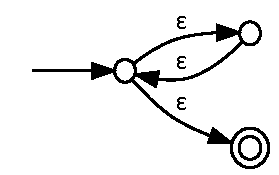
\includegraphics{implementation/inf_loop_simple.pdf}
    \label{fig:inf_loop_simple}
  }
  \subfigure[\textsf{(()())*}]{
    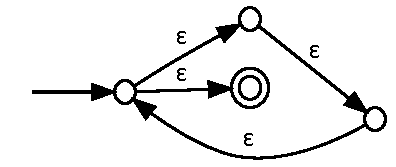
\includegraphics{implementation/inf_loop_long.pdf}
    \label{fig:inf_loop_long}
  }
  \subfigure[\textsf{(\textbar )*}]{
    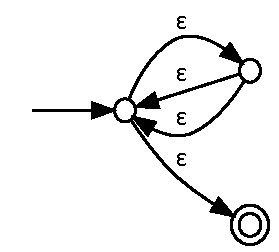
\includegraphics{implementation/inf_loop_many.pdf}
    \label{fig:inf_loop_many}
  }
\caption{$\upvarepsilon$-cycles}
\label{fig:inf_loop}
\end{figure}


From \cite{Cormen} we have the depth-first search (DFS)
algorithm. This algorithm can be modified to detect cycles. In short
it works by initially marking all vertexes white. When a vertex is
encountered it is marked gray and when all its descendants are
visited, it is marked black. If a gray vertex is encountered, then we
have a cycle and do not need to explore further on this path. The
algorithm terminates when all vertexes are black. The algorithm will
terminate, as we color one vertex each step and we always color the
vertexes darker.

To see why this algorithm detects cycles, suppose we have a cycle
containing vertex $a$. Then $a$ is reachable from at least one if its
descendants. When we reach $a$ from this descendant, it will still be
colored gray, since we are not done exploring $a$'s descendants. Thus
the cycle is detected.

Our problem is slightly different: We need to detect if we are in a
cycle of $\upvarepsilon$-transitions. The DFS algorithm solution is
still applicable, with slight modifications, as we do a depth first
search when we explore the $\upvarepsilon$-edges. There will be no
white states. Instead we will have a counter that is incremented every
time a character is read from the input string. Every time a state is
encountered it is stamped with the counter. We can only trust the
color of the state if the counter and the stamp are identical. The
gray and the black states work in much the same way.

In figure \vref{fig:inf_loop} we have some of the NFAs we
encounter. We have an example of a long cycle in figure
\ref{fig:inf_loop_long}, more parenthesis adds more
$\upvarepsilon$-transitions. We also have an example of how more
channels can be created in the loop in figure \ref{fig:inf_loop_many}
by adding alternations. 


\subsection{Filters}

\subsubsection{Groupings}

As we described in section \vref{sec:groupings_filter_analysis}, this
is the filter that should (more or less) throw away any mixed
bit-values not generated in a capturing parenthesis. In order to do
this we need to know which values are generated in a capturing
parenthesis and which are not. We look to Laurikari
\cite{laurikari2001} for inspiration. We will be using a NFA augmented
with extra $\upvarepsilon$-transitions. The extra transitions will be
used to mark the beginning and end of a capturing parenthesis. We will
use the mixed bit-values to navigate the NFA, whenever we are inside a
capturing parenthesis we will copy the mixed bit-values to output. 
\todo[inline]{Add example of the extra epsilon-edges}

We rewrote the regular expression to allow for capturing under
alternation. We will need to insert a \texttt{1} when a group
participates and a \texttt{0} when it doesn't. When exiting the upper
arm of an alternation we need to know how many top level capturing
groups there are in the lower arm and when entering the lower arm we
need to know how many top level capturing groups there in the upper
arm. Again we solve this problem by augmenting the NFA. We insert the
extra information in the split-state marking the entrance to an
alternation and add an extra state at the end of the upper arm.

\todo[inline]{Add example of the extra node and information}

We adopt a similar strategy to solve the problem of reporting only the
first match in capturing under a quantifier. We will again augment the
NFA with necessary information. A state is inserted at the end of the
quantifier, so that this state is the last state that is met in a
iteration of the quantifier. When we pass this state and do another
iteration we will know that we have already been there at least once
and should not output any more bit-values.

\todo[inline]{Add example of star iteration count thingy}


We could also have solved the problem of keeping track of how many
times we have matched a quantifier by simply rewriting the regular
expression. For example would we rewrite \textsf{(a)*} to
\textsf{(\textbar a)a*}. This was dropped because it can not be done
easily on the fly by the NFA generator. The fragment formed by
\textsf{(a)} could no longer be considered a finished fragment that
was just plugged into the rest. We use it with and without the
capturing parenthesis in the rewrite and would therefore need to open
up the fragment and remove the capturing parenthesis for parts of the
rewrite.

%% \paragraph{Capturing under repetition} When using a capturing
%% subpattern, it can match repeatedly using a quantifier. For example
%% matching \textsf{(.)*} with the string \textsl{abc}, the first time we
%% apply the \textsf{*} we capture a \textsl{a} the second time a
%% \textsl{b} and the last time a \textsl{c}. In such a case we have
%% several options when reporting the strings that was captured:
%% \begin{itemize}
%% \item The first
%% \item The last, this is the what most backtracking engines like Perl
%%   do
%% \item All
%% \end{itemize}
%% Only two of these options are available to a streaming filter: All and
%% the first. In order to return the last match, we would have to save
%% the latest match when matching with the quantifier, it is potentially
%% the last and we can not know until we are done matching with the
%% quantifier.

%% Returning all of the strings that were captured is by far the easiest,
%% no extra work is required. On the other hand if we only want to return
%% the first of the matches, we need to know whether or not to return a
%% particular match, that is if this is the first time we match with the
%% quantifier or not. If we alter the way we construct the NFA, we can
%% achieve this. 


%% \paragraph{Capturing under alternation}
%% We are also faced with a choice when values are alternated in a
%% capturing subpattern.


\subsubsection{Trace}

We will limit this filter to only output one channel with a match. In
the current system this is not actually a limitation, as we are using
Thompsons method for matching, there will only ever be one channel
with a match.

All channels are read and the bit-values are saved separately. Every
time we read a channel-split operator we will have to allocate a new
chunk of memory and copy the bit-values we have accumulated up to this
point. When the chunk of memory becomes to small, we will enlarge to a
chunk twice the size. When we reach the end of the input stream, we
will know if there is a match and be able to output the bit-values
that make up the match.


\subsubsection{Serialize}
  
This is the filter that outputs what is matched. We will need the
regular expression, that matches the bit-values, to form the NFA. The
NFA is traversed using the bit-values. As we go along we output the
symbols the transitions are marked with and the escaped symbols in the
bit-values. This should result in a string being outputted of what was
matched.


\section{Conclusion}


\bibliographystyle{plain}
\bibliography{library}

\end{document}
